\documentclass[crop=false,fleqn]{standalone}
\usepackage{../../../globle-preamble}

\begin{document}
    \textbf{Find the domain and range of the funtion $g$ and sketch graph of $g$.}

    $$ g(x) = 
    \begin{cases}
        x-1 &, x < 3 \\
        2x+1 &, x \ge 3
    \end{cases}
    $$

    \vspace{1em}
    Domain of $g(x)$ = $\mathbb{R}$

    Rang of $g(x)$ = $\mathbb{R}$
    \vspace{1em}

    \begin{center}
        \begin{tabular}{ |c|c|c|c|c|c|c|c| } 
            \hline
            $x$ & -1 & 0 & 1 & 2 & 3 & 4 & 5 \\ 
            \hline
            $g(x)$ & -2 & -1 & 0 & 1 & 7 & 9 & 11 \\
            \hline
        \end{tabular}
    \end{center}

    \begin{center}
        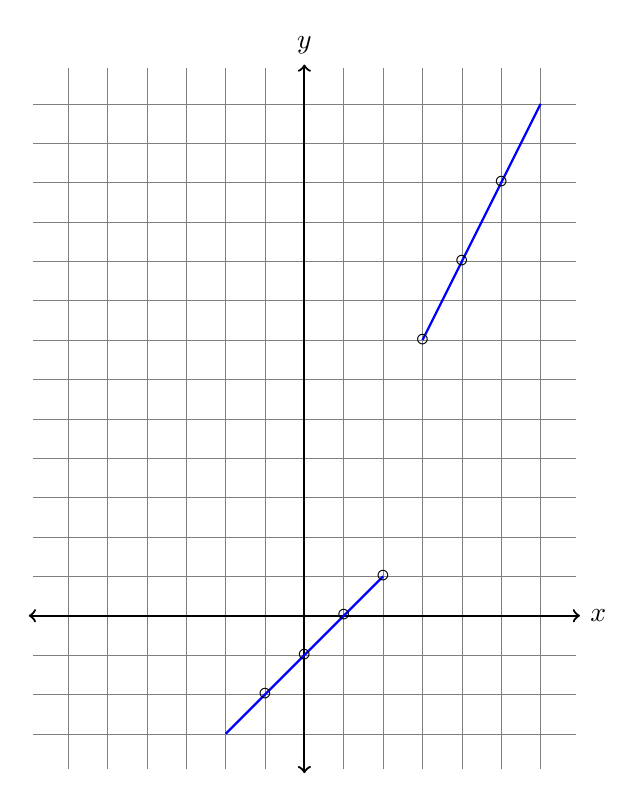
\begin{tikzpicture}[scale=0.5]
            \draw[step=1,gray,very thin] (-6.9,-3.9) grid (6.9,13.9);
            \draw[<->,thick] (-7, 0) -- (7, 0) node[right] {$x$};
            \draw[<->,thick] (0, -4) -- (0, 14) node[above] {$y$};
            
            \draw[domain=-2:2, smooth, variable=\x, thick, blue] plot ({\x}, {\x-1});
            \draw[domain=3:6, smooth, variable=\x, thick, blue] plot ({\x}, {2*\x+1});

            \foreach \Point in {(-1,-2), (0,-1), (1,0), (2,1), (3,7), (4,9), (5, 11)}{
                \node at \Point {$\circ$};
            }
        \end{tikzpicture}
    \end{center}
\end{document}
